\subsection{Scaling of the MG Solver}
	One of the aims of building a parallell multigrid solver was to be able
	to enable simulating large plasma problems. To be able to achieve that the solver
	should be able to scale up very well, i.e. doubling the problem size and the number
	of available processors should only give a manageable increase in computational time.
	We don't expect to be able to achieve a perfect parallelization, since there is
	a certain amount of interprocessor communications necessary that will slow down
	the algorithm compared to a sequential algorithm. The exact parallel performance
	is also dependent on the communications channels and the topology between the processor clusters.
	In \cref{sec:para_comp} the parallel
	complexeties for the different multigrd algorithms is given and we will look at
	the parallel proprties for a V, W and FMG algorithm.


	To investigate the scaling properties we will run set up a standard problem,
	and solve it with increasing resolutions. We start with a \(64^3\) grid on
 	\(1^3\) computaional core, then we increase the problemsize to \(128^3\) on \(2^3\)
	and so on. These tests were run on Abel, UiO's computer cluster, and the technical details
	can be found at the web page \citep{_more_????}.
	%
	%
	\begin{figure}{\textwidth}
		\label{fig:scalingMG}
		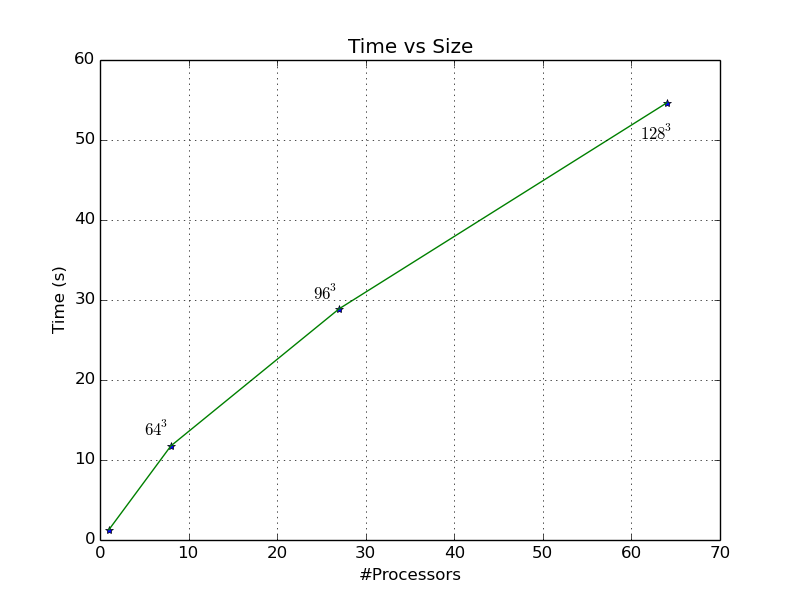
\includegraphics{figures/performance/scalingMG}
		\caption{A Langmuir Oscillation were performed for \(10\) timesteps with a \((32,32,32)\) grid on each processor.
		This was repeated with increasing amount of processors, \((1, 8, 32, 64)\), to see how the multigrid solver scales.}
	\end{figure}
	%
	%Comments
